%%%% ijcai11.tex

\typeout{IJCAI-13 Instructions for Authors}

% These are the instructions for authors for IJCAI-13.
% They are the same as the ones for IJCAI-11 with superficical wording
%   changes only.

\documentclass{article}
% The file ijcai13.sty is the style file for IJCAI-13 (same as ijcai07.sty).
\usepackage{ijcai13/ijcai13}
\usepackage{graphicx}
\usepackage{algorithmic}
\usepackage{algorithm}
% Adaptation au français
\usepackage[utf8]{inputenc}

% Use the postscript times font!
\usepackage{times}
% Package pour faire une flèche
\usepackage{textcomp}


\title{Rapport de projet}
\author{Théo Q, Corto C, Brandon FL \\
Université de Nice\\
France}

\begin{document}

\maketitle


\begin{abstract}
Dans ce projet nous étudions l'impact de la proportion de fourmis chercheuse et ramasseuses dans une fourmilière sur la récolte de nourriture. Nous utilisons pour cela un algorithme de type "Ant colony optimization" en Netlogo. Nos fourmis recherchent des tas de nourritures plus ou moins éloignés et utilisent des phéromones pour les localiser. Nous avons obtenus des données expérimentales en faisant varier graduellement la répartition des fourmis au sein de la fourmilières. Ces données ont ensuite étés  étudiés avec le logiciel R pour extraire un modèle mathématique. L'analyse de la fonction résultats, tempsDecouvertesTas(ProportionChercheuse) donne la répartition optimale :  !-AJOUTER-!
\end{abstract}
\section{Introduction}
\subsection{Contexte}
Les "Algorithmes de colonies de fourmis", "ACO" en anglais, forment une catégorie d'algorithmes d'optimisation basés sur la modélisation d'une colonie de fourmis. En effet bien qu'ayant des capacités individuelles limités ces insectes arrivent collectivement à des solution optimales de problèmes complexes. 



Dans le cadre de l'UE "Projet Scientifique Informatique nous avons choisi le sujet "Colonie de fourmis" d'étude parmi de nombreux proposés. Le modèle de base contenait un seul type de fourmis et trois tas de nourritures fixes. Nous l'avons alors perfectionné.
\subsection{Etat de l'art}
L'ACO est de plus en plus utilisé aujourd'hui dans de très nombreux domaines. Plus particulièrement dans les domaines suivants : planification, routage réseau, affectation, ensembles, conception de circuit nanoélectroniques, traitement d'image etc. Tout les problèmes pouvant se ramener a la recherche d'un chemin optimal dans un graphe en général.
\subsection{Questions scientifiques}
\section{Modélisation}
Pour notre projet nous avons réalisé une simulation via l'outils NetLogo. NetLogo étant un programme de modélisation d'environnement multi-agent. Nous nous sommes appuyé sur un model de base déjà existant proposer par le MIT dans le cadre d'un projet de Mathematique.

\subsection{Hypothèses simplificatrices}
Dans la nature, les fourmis suivent plusieurs critères pour retrouver leurs chemin vers le nid. Elles s'orientent notamment en gardant la trace de la direction, la distance parcourue ainsi que des repères visuels pour retrouver le chemin vers leurs nids. Dans notre modélisation, nous prendrons donc en compte uniquement les pheromones pour retourner au nid. De plus, les fourmis qui ne suivent pas de phéromones suivront un mouvement totalement aléatoire jusqu'à trouver des phéromones.

\subsection{Description du modèle}
Dans un premier temps nous avons créé un nouveau type de fourmis, les fourmis chercheuses. Dans la version de base, le modèle présentait qu'un type de fourmis ne reflétant pas la réalitée. Or, dans notre nouveau modèle, les fourmis ramasseuses se concentrent maintenant exclusivement sur la collecte de la nourriture pendant que les fourmis chercheuses posent les phéromones. Ce modèle est beaucoup plus proche de la réalitée car maintenant, les fourmis se concentrent vraiment sur un tas à la fois en prenant le tas le plus proche.
\begin{figure}[h]
\centering
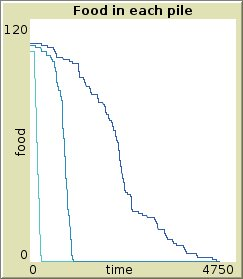
\includegraphics[scale=0.6]{contenue/2antstype.jpg} 
\caption{Proportion de nourriture en fonction du temps}
\label{fig:Tas}
\end{figure}
De plus, notre modèle comprend 4 variables modifiables dont 2 pour la modification de la population. En effet, la variable "Population" nous permet de modifier le nombre de fourmis au total qui sont présentent dans notre fourmilière pendant que la variable "pourcentage" calcul le nombre de fourmis chercheuses en fonction de la population totale (voir les explications de ce choix ici \ref{pourcentage}). De plus, nous sommes dans la capacitée de modifier en direct le pourcentage de diffusion ainsi que le pourcentage d'évaporation des phéromones.
\section{Simulation}
\subsection{Cadre expérimental}

%reference a l'explication des pourcentages
\label{pourcentage}

\subsection{Protocole expérimental}
\section{Résultats}
\section{Discussion}
\section*{Conclusion et perspectives}

\end{document}
